% !TeX spellcheck = en_GB
\section{Simulation}

\subsection{Simulation = Modelling}

It's not possible to simulate something without a model.

\paragraph{Modelling}\mbox{}\\
Deriving calculation schemes (models) where the output variables can
predicted sufficiently accurately from the input variables.

\subsubsection{Finding a model}

One way is to play with the real system to find out how it works and
reacts. If this is possible and the possible damage is low, it might be
a good idea. If the damage is big, it is better to recreate a \textbf{physical
model} (e.g. a big pool to simulate a lake).\\
If this is also not possible one must consider a computer model, which
can be derived from theory (\textbf{Theorie-based model}) or based on
historical data (\textbf{Data-based model}).

\begin{figure}[H]
\centering
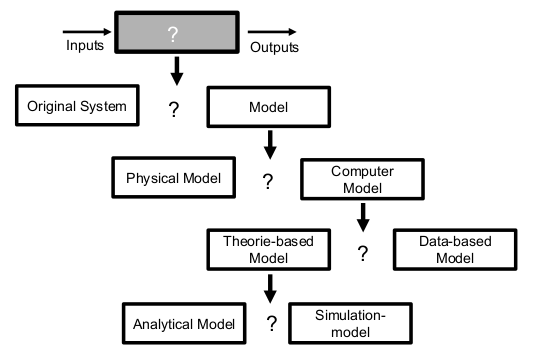
\includegraphics[width=0.7\textwidth]{figures/system_analysis_landscape.png}
\caption{System analysis landscape}
\end{figure}

\subsection{Different simulation paradigms}

\begin{description}
	\item[Monte Carlo Simulation] MC Simulation is a broad class of algorithms
	that rely on repeated sampling to obtain numerical results.
	\item[System Dynamics] SD is an approach for understanding the behavior of
	complex systems over time, using stocks, flows, feedback loops, and time
	delays.
	\item[Discrete event simulation] Simulation, where system state only changes
	at discrete points in time.\\
	Key element: Queue.
	\item[Multi-agent simulation] In MA Simulation, we have a system that
	consists of multiple entities with identical or different behaviour.
	They solve problems collectively.
\end{description}

\subsection{Monte Carlo simulation}

MC Simulation is a numerical method for statistical simulation. It is
based on using sequences of random numbers in order to explore the
behaviour of the system. Monte-Carlo simulation also provides an
alternative for solving complex problems in probability and statistics.

\subsubsection{Properties}

\begin{itemize}
	\tightlist
	\item MC Simulation is a powerful instrument for complex statistical
	analysis which helps compute probabilities and probability
	distributions.
	\item It requires a quantitative description of the system.
	\item Virtual experiments with the system are carried out in order to draw
	conclusions about its behavior.
\end{itemize}


\subsubsection{Monte Carlo Model}

\begin{figure}[H]
\centering
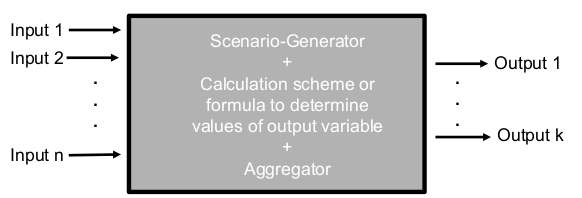
\includegraphics[width=.75\textwidth]{figures/montecarloModel.png}
\caption{Monte Carlo Model}
\end{figure}

\begin{itemize}
	\tightlist
	\item The Scenario-Generator creates scenarios according to a prescribed
	probability distributions that match reality.
	\item Each scenario yields values of the target variable that can be
	obtained via a calculation scheme or formula.
	\item The Aggregator calculates the output(s) form the target values
	associated with each simulated scenario.
\end{itemize}

\subsection{Discrete Event Simulation (DES)}

A Simulation-model is a virtual representation of a real-world system
that allows to gain insights in how the system works in reality.

\begin{figure}[H]
	\centering
	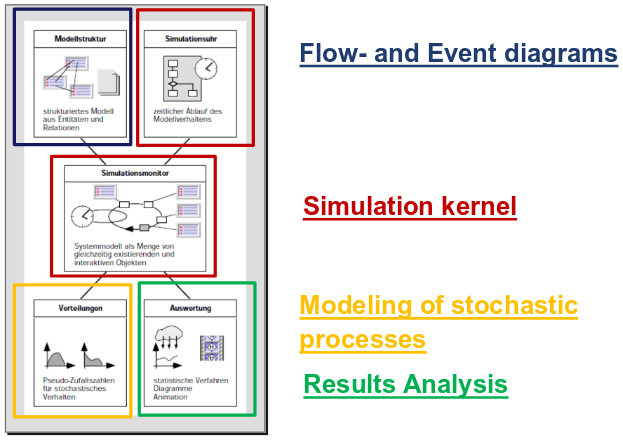
\includegraphics[width=.85\textwidth]{figures/overviewDES.png}
	\caption{Overview DES}
\end{figure}

\subsubsection{Characteristics/properties}

\begin{itemize}
	\tightlist
	\item Presence of stochastic (random) variables.
	\item (Evolution over) Time plays an important role.
	\item Individual entities are being monitored (in contrast do SD).
	\item State changes are the result of "events". Events only take place a
	discrete points in time.
	\item DES successfully applied in many different environments like shop
	floor control, spare parts logistics, pedestrian modelling, et cetera.
	\item Key element in DES: Queueing system.
\end{itemize}


\subsubsection{Queuing System}

In a queuing system, \textbf{jobs} are processed by a \textbf{server}.
Under the (realistic) assumption that the server has a particular
limited capacity (e.g. specified as the maximum number of jobs that can
processed per hour), the system can get congested and waiting times may
occur.

\mbox{}\\
Interesting properties of a queuing system are:
\begin{itemize}
	\tightlist
	\item Stability of the system.
	\item Number of customers in queue.
	\item Average waiting time.
	\item 95\% percentile of all waiting times.
	\item ...
\end{itemize}

\subsubsection{Advantages}

\begin{itemize}
	\tightlist
	\item Cost-effective, fast, and safe field of experimentation (compared to
	experimenting with original system).
	\item Allows animation and hence increases system understanding.
	\item Allows the analysis of complex systems at a high level of detail
	(compared to analytical solutions)
\end{itemize}


\subsubsection{Disadvantages}

\begin{itemize}
	\tightlist
	\item Requires significant (software) development time.
	\item Construction of a simulation model is relatively prone to error.
	\item Sound interpretation of results is challenging.
\end{itemize}

\subsubsection{Key Elements}

\begin{description}
	\item[Items (or entities)] Items that flow through the system.\\
	Examples: Patients, Spare parts, Production orders, Cars, et cetera.\\
	\emph{Items usually have attributes.}
	\item[Simulation clock] Virtual time within the simulation model.
	\item[System state] The state $Z(t)$ gives a full description of the system
	at time $t$.
	\item[Future event list] Dynamic list that contains 0 or more (time, event)
	pairs.\\
	It contains those events that are known at the current time of the
	simulation clock. During a simulation run , events are added and
	removed from this list continuously.
	\item[Event] Each event has an effect at the time of occurrence. The effect
	consists of a change to \textit{the system state} and/or a change to the
	\textit{Future Event List}.\\
	In the time between two consecutive events, nothing happens (the
	system state remains unchanged). Therefore the simulation clock can
	jump from event to event.
\end{description}


\subsection{Flow- and Event Diagrams}

Discrete Event Simulation Models are specified through Flow- and
Event Diagrams. They show how items can move through the system.
To do this, they use:

\begin{itemize}
\tightlist
\item Attribute values of active items
\item System state
\item Future Event List
\end{itemize}


\subsubsection{Building Blocks}

\begin{figure}[H]
\centering
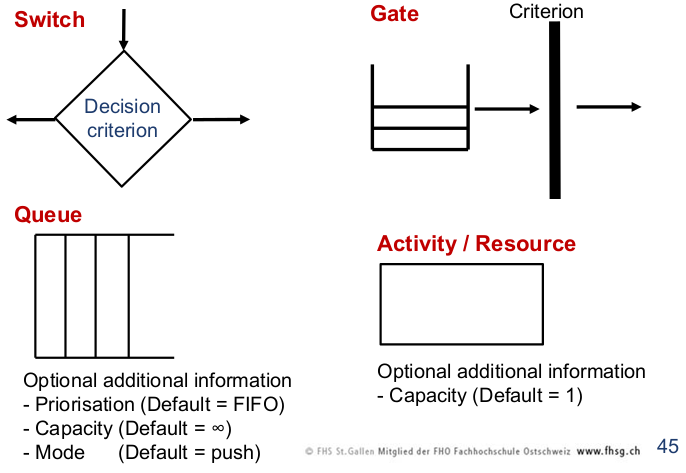
\includegraphics[width=0.5\textwidth]{figures/flowDiagramBuildingblocks1.png}
\caption{Building Blocks 1}
\end{figure}

\begin{figure}[H]
\centering
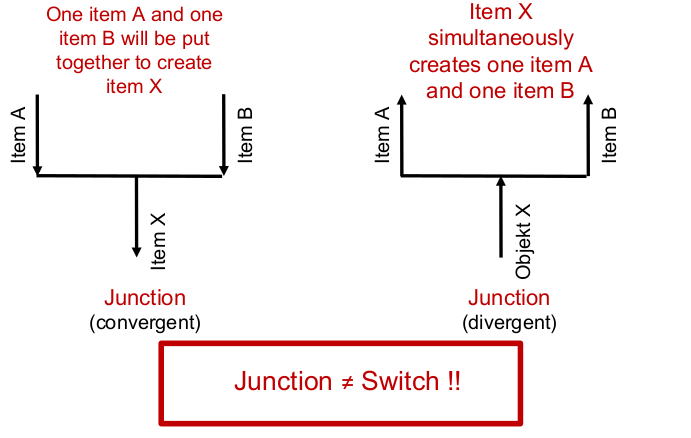
\includegraphics[width=0.5\textwidth]{figures/flowDiagramBuildingblocks2.png}
\caption{Building Blocks 2}
\end{figure}

\begin{figure}[H]
\centering
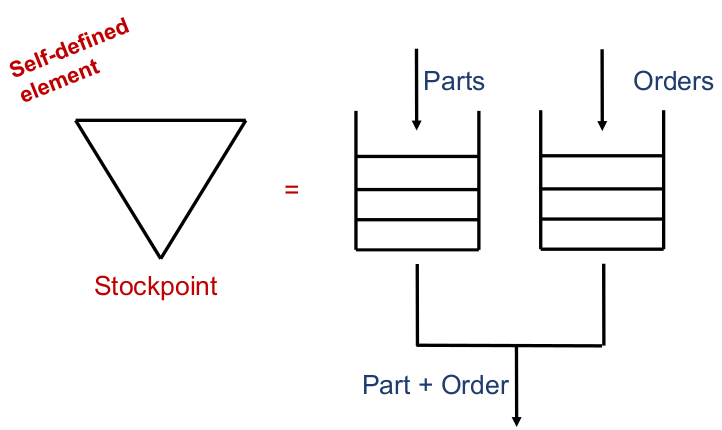
\includegraphics[width=0.5\textwidth]{figures/flowDiagramBuildingblocks3.png}
\caption{Building Blocks 3}
\end{figure}

\subsubsection{Best practices}

\begin{itemize}
	\tightlist
	\item Avoid intersecting arrows.
	\item Add small explanations to arrows, resources and activities.
	\item Consider building sub-models if the number of visual components get
	bigger than $\approx10$.
\end{itemize}


\subsection{DES Simulation}

\subsubsection{Event-diagram}

The event-diagram is used in DES simulation to simulate a DES model.

\begin{figure}[H]
	\centering
	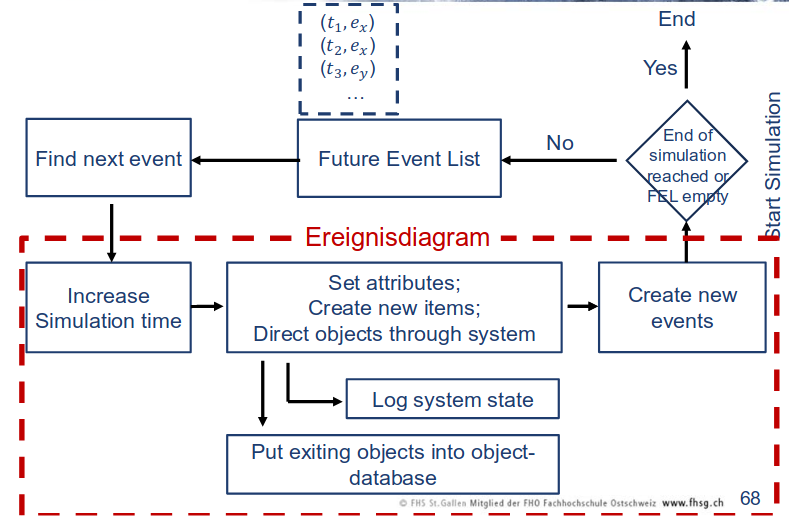
\includegraphics[width=.5\textwidth]{figures/ereignisdiagram.png}
	\caption{Example of an event-diagram}
\end{figure}


\subsubsection{DE Mechanics}

\begin{figure}[H]
	\begin{subfigure}{\textwidth}
		\centering
		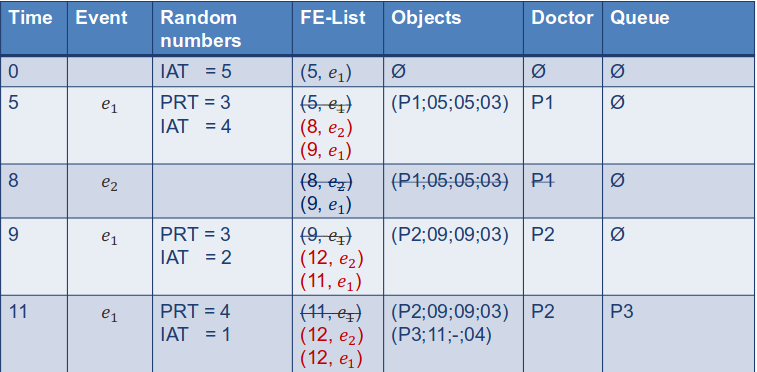
\includegraphics[width=.8\textwidth]{figures/DEMech1.png}
	\end{subfigure}
	\begin{subfigure}{\textwidth}
		\centering
		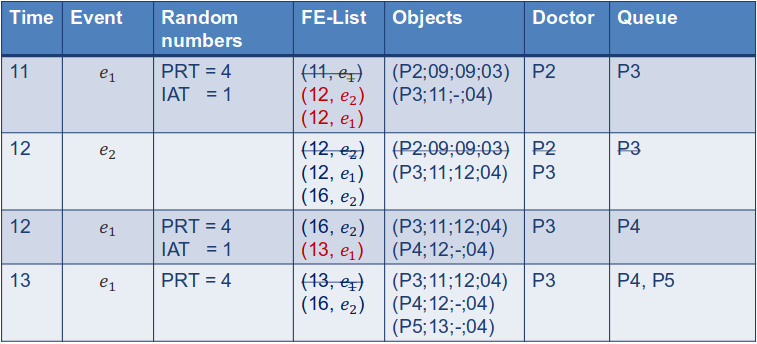
\includegraphics[width=.8\textwidth]{figures/DEMech2.png}
	\end{subfigure}
	\begin{subfigure}{\textwidth}
		\centering
		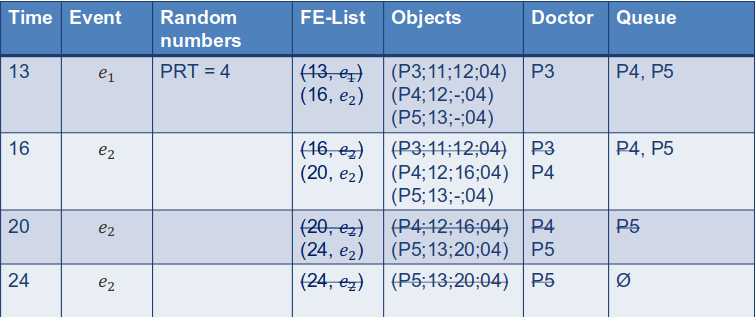
\includegraphics[width=.8\textwidth]{figures/DEMech3.png}
	\end{subfigure}
	\caption{Example event table of a doctor's office.}
\end{figure}

\begin{description}
	\tightlist
	\item [PRT] Process Time (duration of the process)
	\item [IAT] Inter arrival time (time until next event/arrival)
	\item [FE-List] Time of next event
	\item [Objects] Current Working state
	\item [Queue] Waiting list
\end{description}

\subsection{Stochastic processes}

When modelling processes random variables are often use to define PRTs
and IATs or any other value.

\subsubsection{Random variables}

In statistics, uncertainties are modelled via random variables.\\
A random variable is a numerical value assigned to the possible outcomes
of a chance experiment.

These properties must be set for each random variable:

\begin{itemize}
	\tightlist
	\item \textbf{Distribution type}
	\begin{itemize}
		\tightlist
		\item Theoretical distribution (Uniform, Exponential, Normal)
		\item Empirical distribution (Sampling from historical data)
	\end{itemize}
	\item Estimating parameter values in selected probability distribution
\end{itemize}

\subsubsection{Theoretical distributions}

\begin{figure}[H]
	\begin{subfigure}{\textwidth}
		\centering
		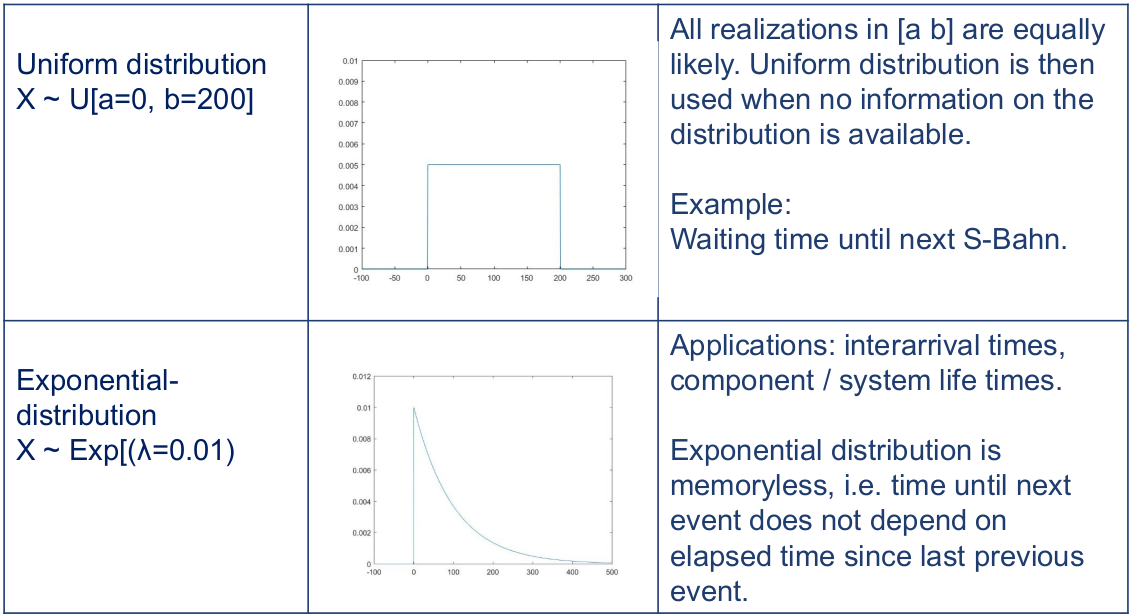
\includegraphics[width=.7\textwidth]{figures/TheoreticalDistributions1.png}
	\end{subfigure}
	\begin{subfigure}{\textwidth}
		\centering
		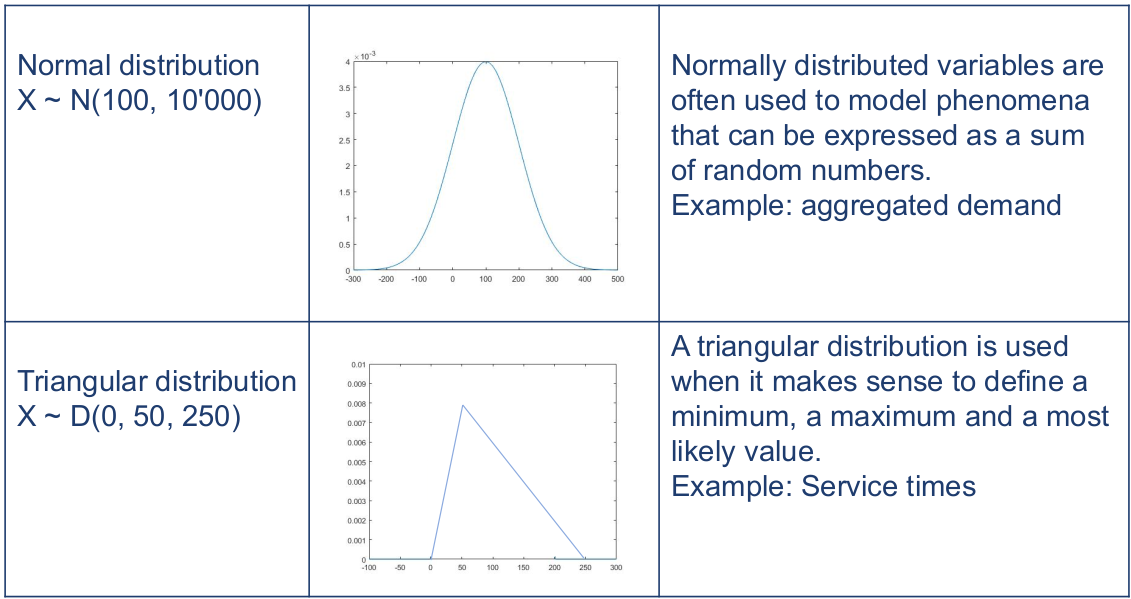
\includegraphics[width=.7\textwidth]{figures/TheoreticalDistributions2.png}
	\end{subfigure}
	\caption{Different theoretical distributions}
\end{figure}

\paragraph{Advantages of theoretical distributions}
\begin{itemize}
	\tightlist
	\item Compact formulations (usually 1 or 2 parameters)
	\item Easy to adjust (via small number of parameters)
	\item Wide range of returned random numbers
\end{itemize}

\paragraph{Disadvantages of theoretical distributions}
\begin{itemize}
	\tightlist
	\item Limited number of parameters for adjusting the distribution in the
	desired direction. It may just not be possible to describe reality via a
	probability distribution with 1 or 2 (or 3) parameters.
\end{itemize}

\subsubsection{Empirical distribution}
An empirical distribution represents the same probability for value X as
in real historical data.

\paragraph{Advantages of empirical distributions}
\begin{itemize}
	\tightlist
	\item Based on real data.
	\item Any shape is possible.
\end{itemize}

\paragraph{Disadvantages of empirical distributions}
\begin{itemize}
	\tightlist
	\item It is not possible to generate (random) numbers that have not already
	occurred in the past. This means that we usually need data over a long
	time horizon.
	\item Empirical distributions cannot be described in a compact manner.
	\item High memory footprint
\end{itemize}

\subsection{Modelling stochastic processes}
No matter, if we use theoretical or empirical distributions to model a
stochastic process, there are a few important issues when working with
data that we need to take care of.

\subsubsection{Common mistakes}

\begin{itemize}
	\item Not enough data available for a sound statistical analysis.
	\item No outlier detection / removal and/or data filtering.
	\item Seasonal patterns (summer / winter, Mon-Fri versus Sat-Sun)
	ignored. Example: ER Hospital Davos: February $\ne$ June: one
	(average) arrival rate is not sufficient.
	\item Use of non-representative historical data.
	\item Wrong Interpretation of available data
\end{itemize}

\emph{Always plot the data!}

\subsection{Random generators}

\subsubsection{Requirements}

\begin{itemize}
	\tightlist
	\item Independent (i.e. uncorrelated to previous realizations).
	\item Uniformly distributed.
	\item High resolution (no gaps).
	\item No cycles.
	\item Fast and memory friendly creation.
	\item Reproducibility (seed).
\end{itemize}

The series of random numbers should be reproducible to reproduce
situations.

\subsubsection{Linear congruency method}

Fulfils the above requirements.
\begin{equation}
X_{i+1} = (aX_i+c) \mod m\\
u_i = \frac{X_i}{m-1}
\end{equation}

\begin{itemize}
	\tightlist
	\item $a$, $c$, $m$ and $X_0$ are integers.
	\item $m > 0$
	\item $a < m$
	\item $c < m$
	\item $X_0 < m$
	\item Quality of Randomgenerator strongly depends on $a$, $c$ and $m$.
	\item In particular, a and m are important. Often very big prime numbers
	are used, e.g. $m=2^{32} -1$.
\end{itemize}

In practice, we often need to generate random numbers with distributions
other than the uniform distribution. Next we see how to derive such random
numbers from uniformly distributed random numbers $X \sim U[0 1]$.
We differentiate between discrete and continuous distributions:

\begin{itemize}
	\tightlist
	\item \textbf{Discrete distribution}
	\begin{itemize}
		\tightlist
		\item Interval method
	\end{itemize}
	\item \textbf{Continuous distribution}
	\begin{itemize}
		\tightlist
		\item Inversion sampling
		\item Rejection sampling
	\end{itemize}
\end{itemize}

\subsubsection{Interval method}
Sometimes we need a random generator that returns particular numbers (or
objects), each with its own pre-specified probability.

\begin{figure}[H]
	\centering
	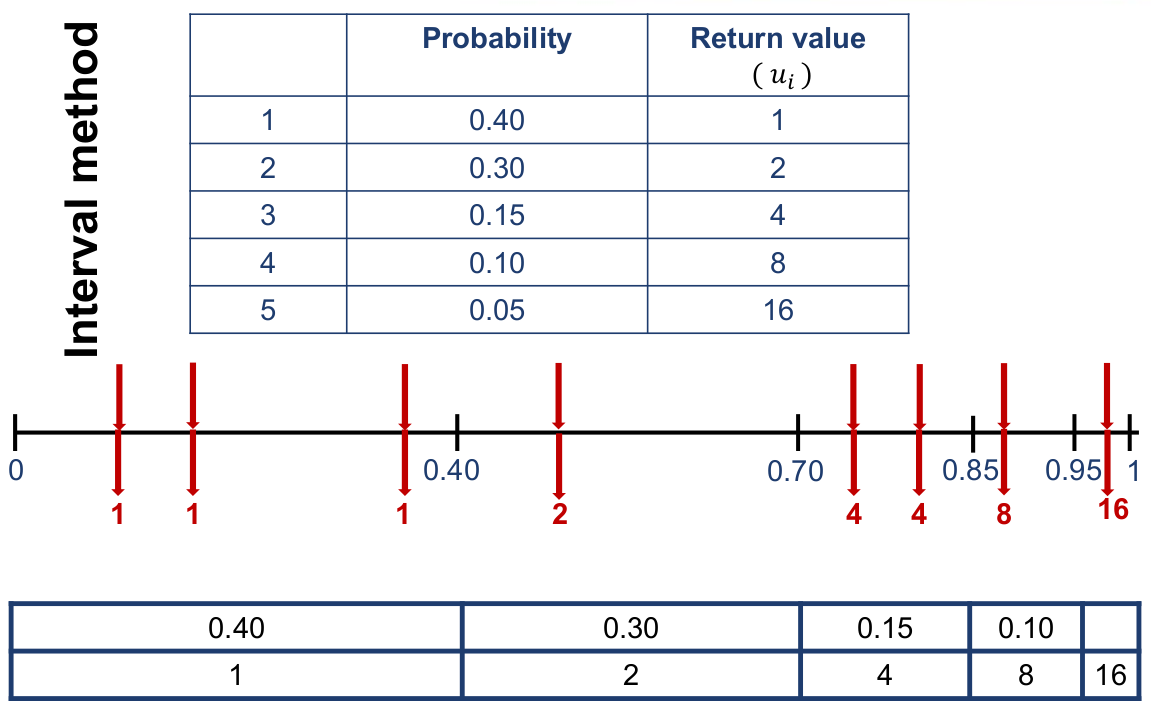
\includegraphics[width=.6\textwidth]{figures/IntervalMethod.png}
	\caption{Example of the interval method}
\end{figure}

\subsubsection{Inversion sampling}
Method to transform standard random numbers into random numbers
that follow a certain given distribution $F()$.

\begin{enumerate}
	\tightlist
	\item Create $x = U[0,1]$
	\item Calculate $y = F^{-1}(x)$
\end{enumerate}

\paragraph{Exponential distribution}
\begin{equation}
F(x) = 1 - e^{-\lambda x}
\end{equation}
\begin{equation}
F(x)^{-1} = -\frac{1}{\lambda}\cdot ln(1-x)
\end{equation}
\begin{equation}
\lambda = \frac{1}{E(x)}
\end{equation}

\subsection{Independent simulation run method}
In this method, multiple simulation runs are carried out, each with its own
random seed. Each simulation run yields one sample mean Xi. By design,
all Xi are uncorrelated. This means that we can apply basis statistics.

\subsubsection{Warm-Up period}
\begin{figure}[H]
	\centering
	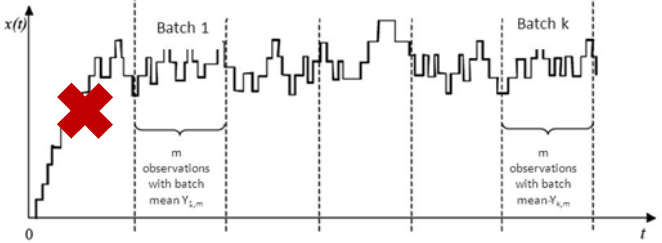
\includegraphics[width=0.7\textwidth]{figures/WarmUpPeriod.png}
	\caption{Warmup Period}
\end{figure}

Most of the times, we are interested in the long-run system behavior.
The simulation run however starts with some system state which might
not be realistic at all (think e.g. idle queuing systems).\\
\\
Consequently, we must remove this warm-up phase from the data
before starting our analysis. We normally have to throw away between 1-2
batches.

\subsubsection{Result Analysis: Batch-Means Method}
After the removal of the warm-up period, simulation time is divided into n
equal intervals. For each interval the mean value for the desired
performance measure is computed.
Under the assumption that the batches are independent (which is the
case if each batch is long enough), the confidence interval for the
estimated parameter can be computed from the empirical variance of the
batch means.

Sample Mean:
\begin{equation}
\hat{\Theta} = \frac{1}{n}\sum_{i=1}^n \hat{\Theta_i}
\end{equation}

Sample Variance:
\begin{equation}
S^2 = \frac{1}{n-1}\sum_{i=1}^n (\hat{\Theta_i} - \hat{\Theta})^2
\end{equation}

Confidence Interval:
\begin{equation}
[\hat{\Theta}-z_{\alpha/2}\cdot \sqrt{S^2/n};
\hat{\Theta}+z_{\alpha/2}\cdot \sqrt{S^2/n}]
\end{equation}

\begin{figure}[H]
	\centering
	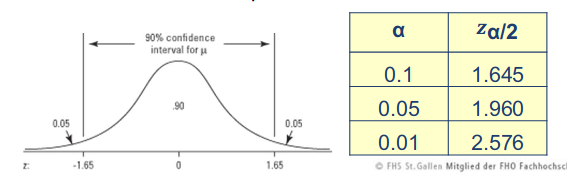
\includegraphics[width=0.7\textwidth]{figures/ConfidenceIntervalValues.png}
	\caption{Common values for $z_{\alpha/2}$}
\end{figure}




\subimport{.}{06_SimulationOptimization}
